\section{WATER!}

\margininbox{M2}{
     \begin{itemize}
    \item Gergely Ambrus
    \item Paul Hutton
    \end{itemize}}{\explo}

It was one of the last pushing trips on the expo. Once again, we decided
to go down to the unpassable rift at the bottom of \passage{M2} in order to
find the Connection. This time, for sure, it was going to happen! Paul
seemed to be as eager as I was, so we teamed up.


\tweet{2:32PM Aug 10th, 2008}{\protect\passage{S1}: way to right hand pitch found by hammering rift above big pitch.Strong draft from tight meander, several hrs hard hammer.4th system?}

At the same time, another party (Jarvist and Dan) was to go down to the
``other side'' of the rift, to hear our voices and then to shake hands,
for sure. So we slowly worked our way down the many tight squeezes below
\passage{Silos}, and arrived at the -- by then, familiar -- small and cosy
chamber. From here, the hammer and the chisel played the main role in
our drama, or at least we thought so.

It was not until a couple of hours later that we noticed that instead of
the usual sound of water dripping into the pool, a steady, loud,
constant noise is coming from the chamber. Squeezing back, we nervously
looked at the stream of water dropping into the pool. Time to head out,
as quick as possible! We threw some small flakes of the chocolate
tinfoil to the stream in order to find it on the other side, hastily
packed up, and started our way up, which turned out to be an ordeal. I
wore a normal textile oversuit, which proved to be perfect for the cold
water to directly run through, but Paul did not feel much better in his
Meander either. \bignote{The cave suddenly became like a wet Yorkshire cave, and
soon we were completely soaked in the icy water}.

The flow became bigger and bigger, and our only hope was that from the
top of \passage{Silos}, the way should be dry, as we have never seen water
there. Yet, once reaching the top, completely cold, exhausted,
shivering, we had the worst sight in front of us: a 40 m high waterfall,
the rope hopelessly dangling in the middle, with the majestic and
frightening sound of water as it splashes at the rocks after its long
freefall\sidenote{believe this is \passage{Kletnikov Skropilnik} AKA Kletnik's Shower}. At this point, there was no choice left: being as cold as we
were, the survival bags would have been almost useless, and the water
level seemed to rising, indicating that it is still raining on the
surface, so did we decide to wait, it would have been at least half a
day, resulting in hypothermia almost surely. We ate the last bits of
chocolate we had, jumped, rubbed our arms to get some blood going,
looked up into to dark, trying to estimate what is awaiting us. Neither
of us was sure that we were going to make it. There was a ledge midway
out of the water, so planned to go up there in one go, and then continue.

\tweet{3:16PM Aug 17th, 2008}{M2:JH/JKP derig via M16, put to sleep for the year. CK:DG/TO last pushing trip to desperately seek the con, morning callout.}

Then, I clipped onto the rope. The jammers were in place, everything
sorted out, feet in the footloop, bag on the back, rope as tight as
possible. It was the moment to start. A wide swing took me directly in
the middle of the water, and without thinking, I started prussiking as
fast as I could. The force of the icy water seemed to be much stronger
than my weak, half-frozen thighs, and it was hard to get any air, like
being in the middle of a freezing icefall. I started swearing, knowing
that I had to win. Seconds seemed minutes, and minutes hours, but
finally I made it to the ledge. Paul could hardly hear the ``rope
free'', then he started up. I crossed my fingers and waited. The
gigantic howling sound covered everything, the shouts of Paul went to
thin air. \tweet{1:42PM Aug 18th, 2008}{GW derigged in full, VILINSKA jama tied in. No connection, but \textasciitilde 1.2km of new cave this year, with fantastic leads for 2009! Team Mig.} Finally, he emerged with a frightened, completely pale face,
blue lips, shivering, his hands are of almost no use at all. We hugged
each other and jumped, trying to warm up. Then, the second half, just as
bad as the first. When Paul showed up at the top, we smiled a bit: from
here, we get out, even if we have to duck all the way! It was still a
good couple of hours until we made it to the surface, about 6 hours
after the callout. We dragged back to camp in the pouring rain, woke up
Tetley, drank a bit of booze, and went for a massive 15 hour sleep --
which was quite well earned after all.

\name{Gergely Ambrus}




\begin{figure*}
      \checkoddpage \ifoddpage \forcerectofloat \else \forceversofloat \fi
      \centering
    \begin{subfigure}[t]{\textwidth}
    \centering
        \frame{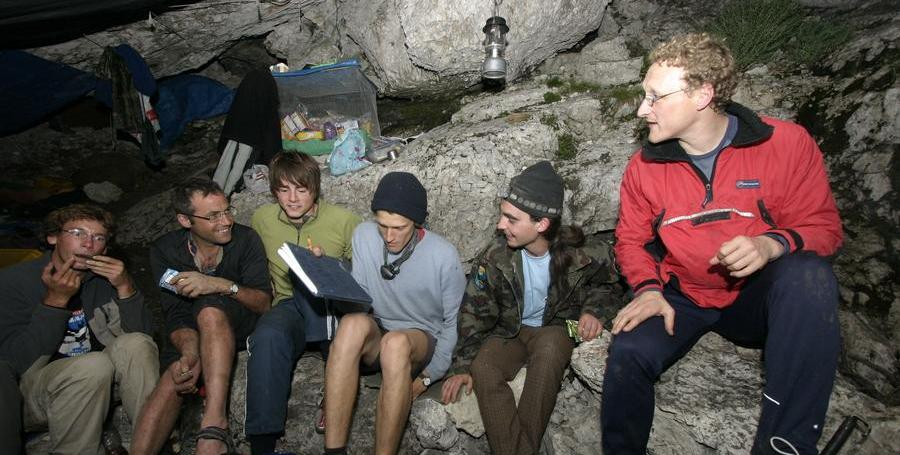
\includegraphics[width=\linewidth]{2008/water/MMslov08 39--orig.jpg}} 
        \caption{\textit{left to right} Gergely Ambrus, Tetley, Paul Hutton, Jarvist Frost, Izi Možir, Jim Evans. \pic{Martin McGowan}} \label{bivi jim}
    \end{subfigure}
    
          \vspace{0.3cm}
          
    \begin{subfigure}[t]{0.49\textwidth}
        \centering
        \frame{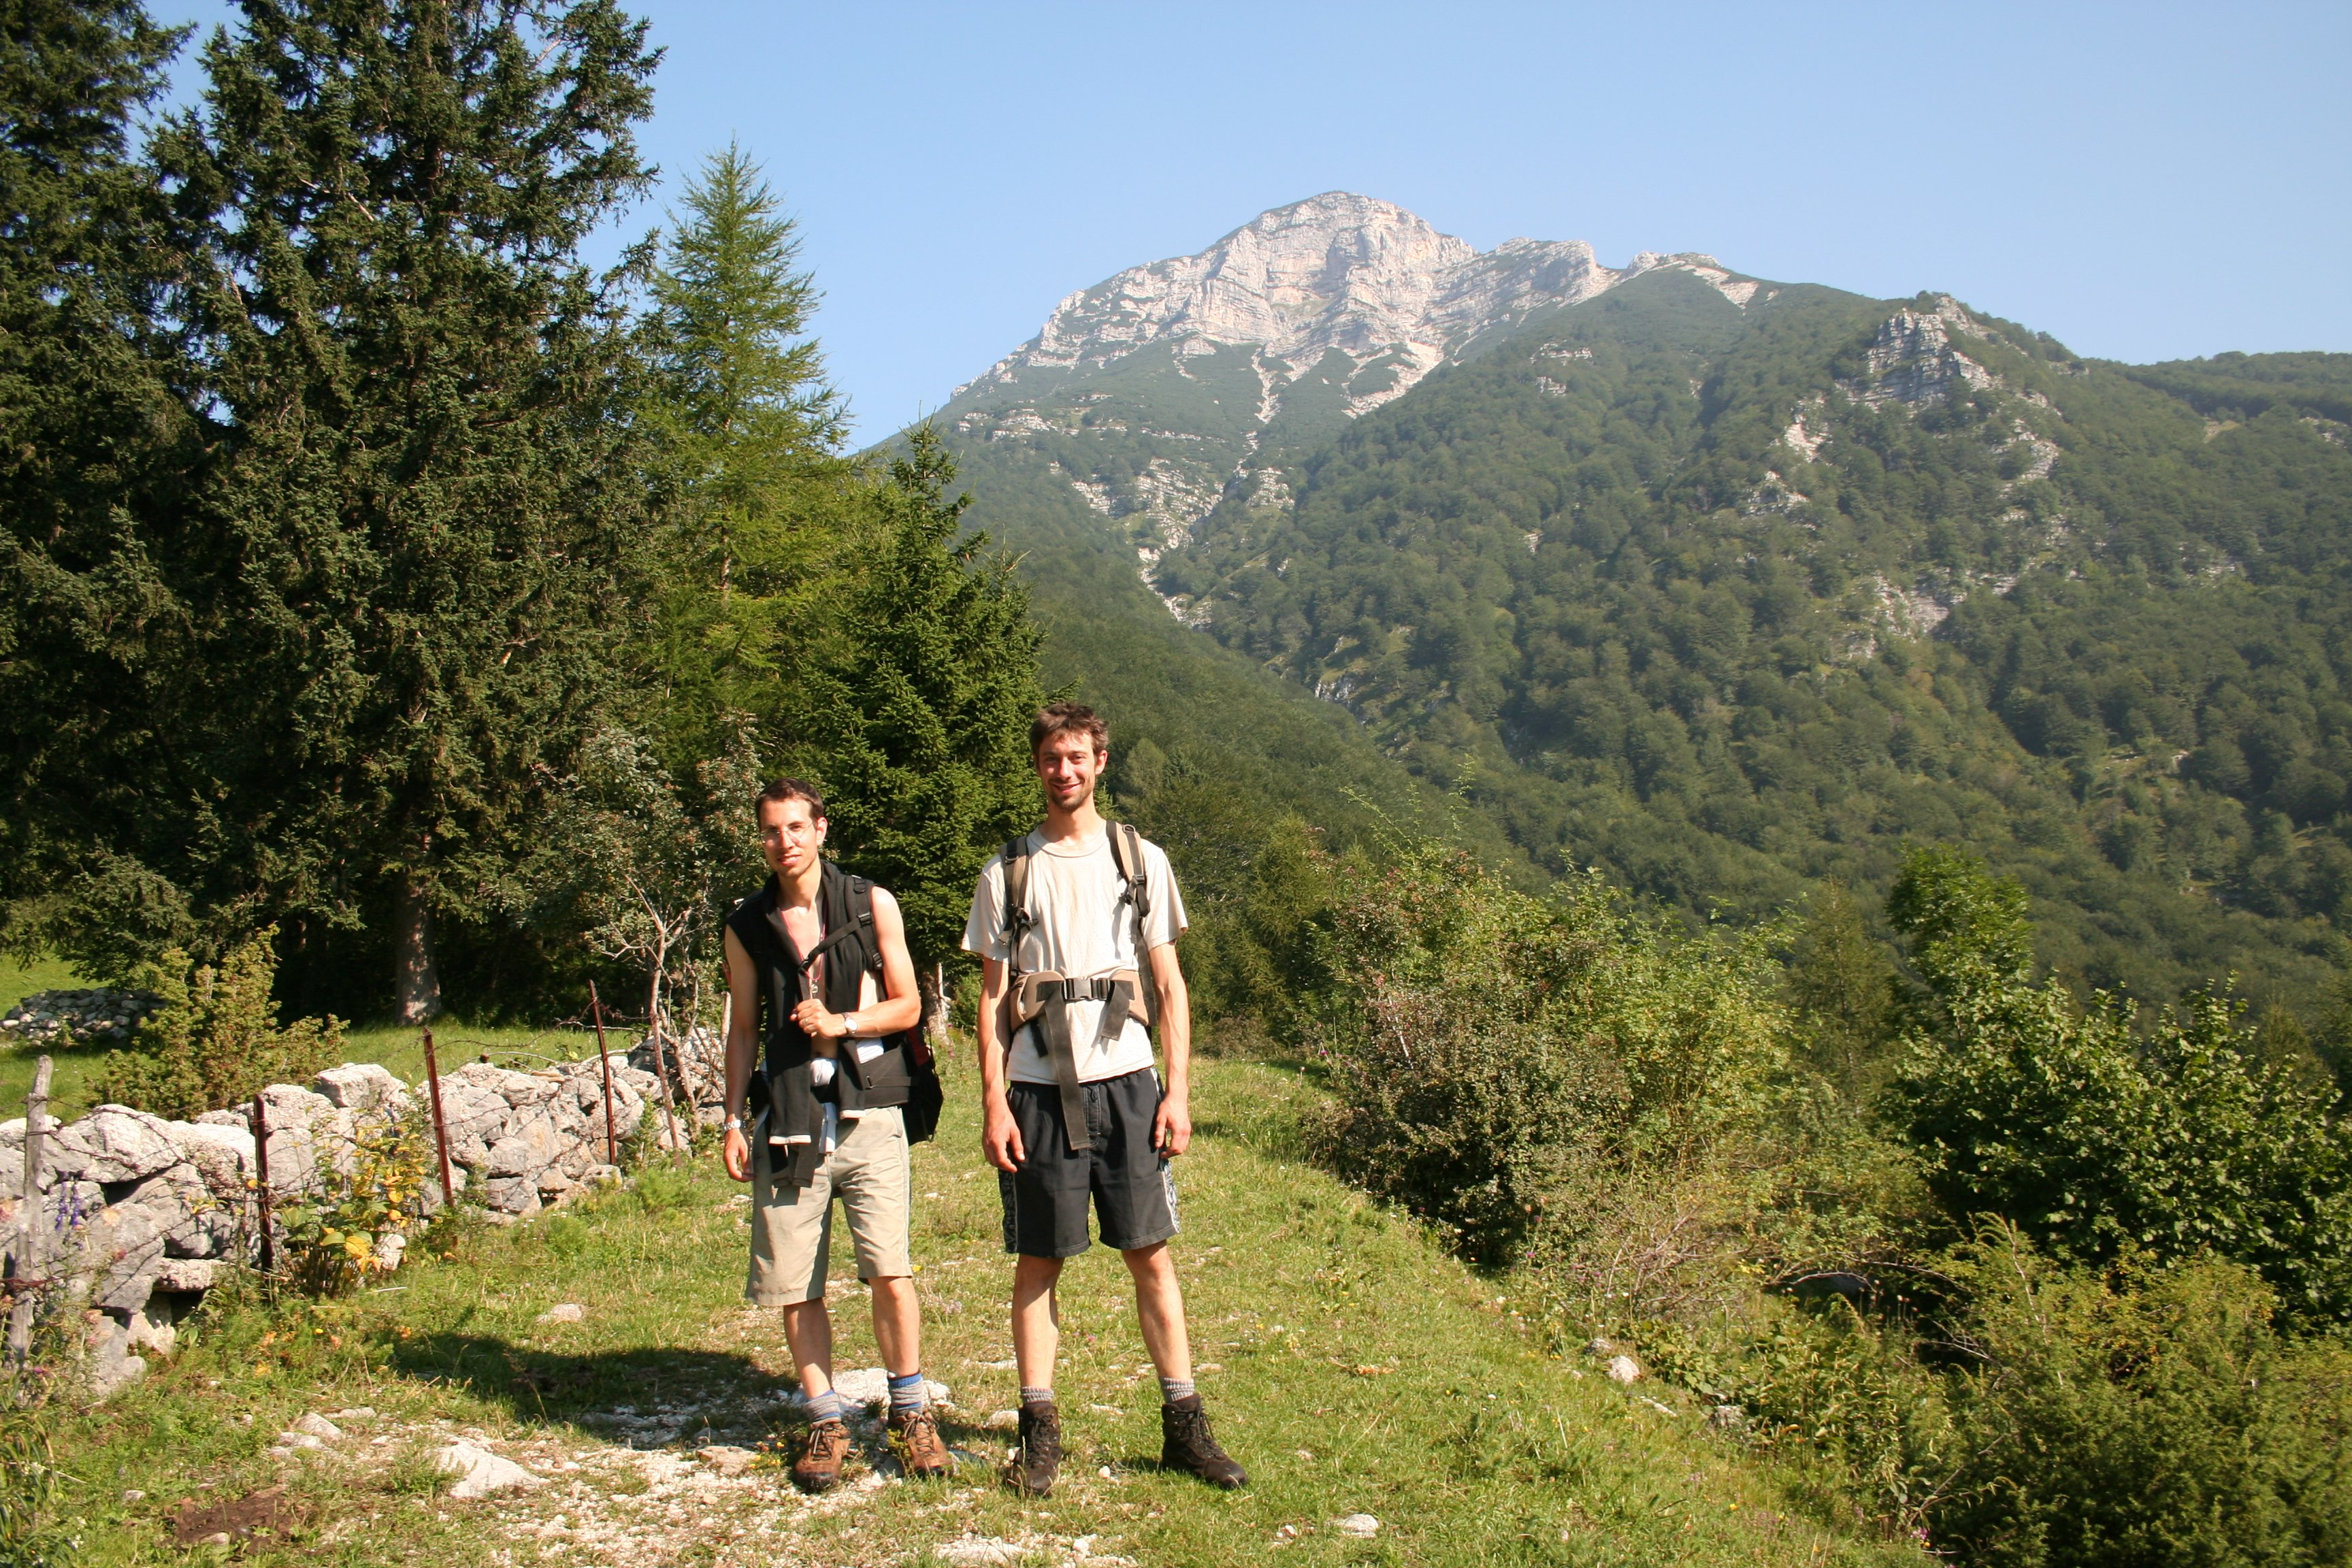
\includegraphics[width=\linewidth]{2008/water/Jana Carga - Canon 350D - img_3189 James Kirkpatrick and Clewing Griffith on start of walk up to Mig with peak behind them--orig.jpg}} 
        \caption{Clewin Griffiths and James Kirkpatrick. \pic{Jana Čarga}} \label{clewin jkp mig}
    \end{subfigure}
    \hfill
    \begin{subfigure}[t]{0.49\textwidth}
        \centering
        \frame{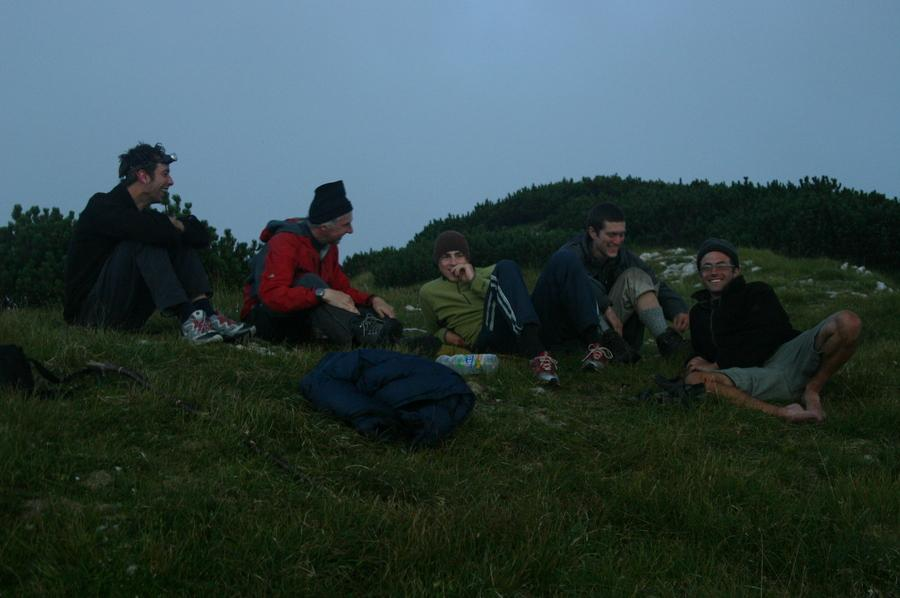
\includegraphics[width=\linewidth]{2008/water/Gergely Ambrus - DSLR - img_4852--orig.jpg}} 
        \caption{\textit{left to right} James Kirkpatrick, Martin McGowan, Paul Hutton, Dan Greenwald, Tetley. \pic{Gergely Ambrus}} \label{sunset lounge}
    \end{subfigure}

    \caption{Some of 2008's team members.}
\end{figure*}
